%version 1.00,	date 24/10/2016	auteur(s) Pierre Porche
\speaker{\Matthieu}

\begin{frame}
\frametitle{Outils techniques de qualité}
\begin{block}{Intégration dans le projet de nombreux outils d'aide au développement}
	\begin{itemize}
		\item SonarQube
		\item PhpCodeSniffer
		\item PhpUnit (avec couverture de code)
		\item PhpDocumentor
	\end{itemize}
\end{block}
\end{frame}

\begin{frame}
      \begin{figure}[r]
		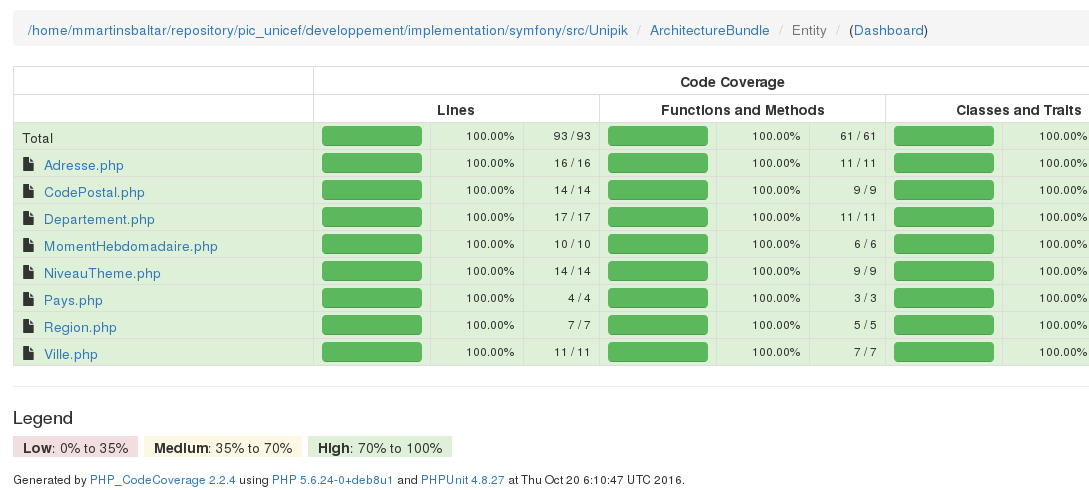
\includegraphics[scale=0.3]{images/coverage.png}
		\caption{Capture d'écran de la couverture des tests}
	  \end{figure}
\end{frame}

\begin{frame}
      \begin{figure}[r]
		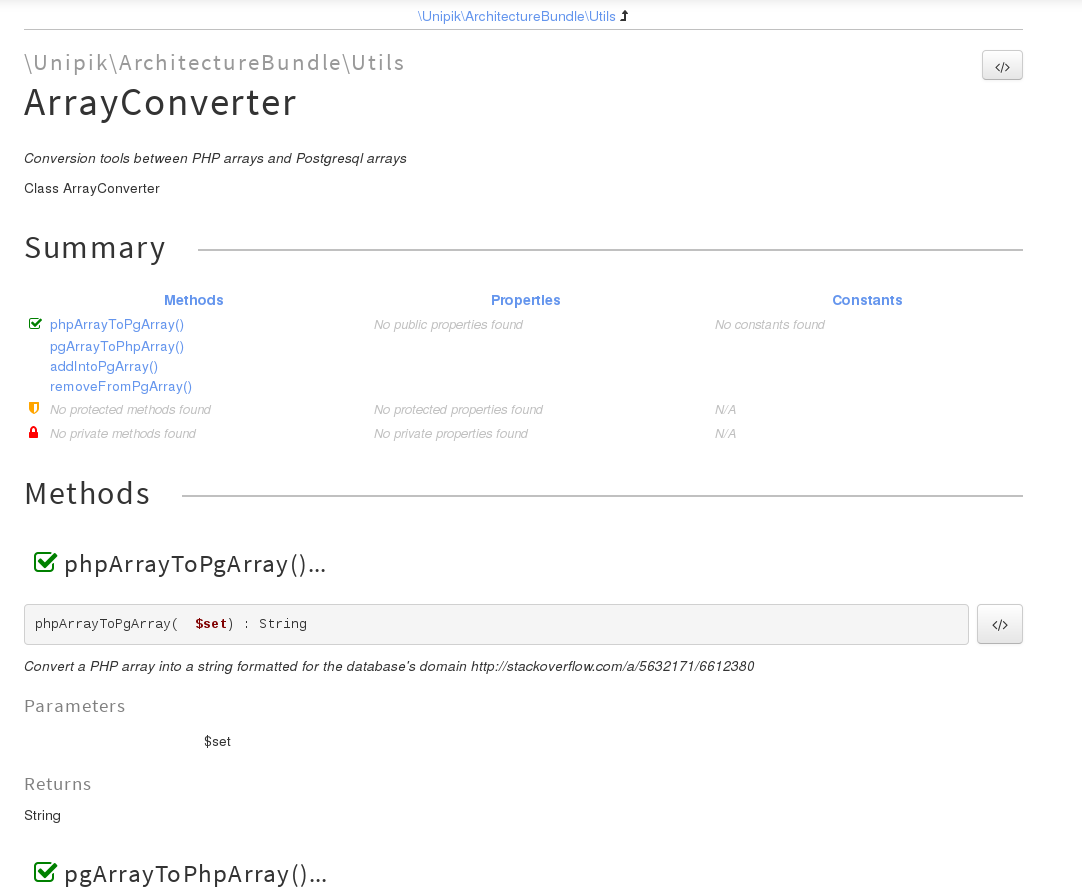
\includegraphics[scale=0.2]{images/doc.png}
		\caption{Capture d'écran de la documentation}
	  \end{figure}
\end{frame}

\begin{frame}
\frametitle{Déploiement automatique}
\begin{block}{Environnements multiples}
	\begin{itemize}
		\item Développement: apache avec symlink vers le dossier de travail \\
		\emph{\tiny(http://prenom.unipik.insa-rouen.fr)}
		\item Intégration: VM sur le pare-feu de la salle PIC (Vagrant) \\
		\emph{\tiny(http://integ.unipik.insa-rouen.fr)}
		\item Pré-production: machine physique dédié dans la salle pic. \\
		\emph{\tiny(http://pre-prod.unipik.insa-rouen.fr)}
		\item Production: chez Digital Ocean (bientôt chez Quantic Telecom) \\
		\emph{\tiny(http://138.68.151.59)}
	\end{itemize}
\end{block}

L'intégration, la pré-production et la production sont approvisionnés automatiquement avec Ansible.

\end{frame}
